\subsection*{The $C_{\sf sparse+latent}$ estimator is most efficient in neural data}
\begin{figure}
\begin{fullpage}
        \begin{center}
        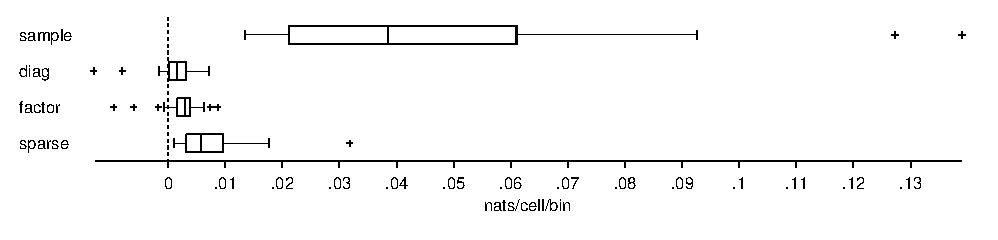
\includegraphics[width=\textwidth]{./figures/Figure3.eps}
        \end{center}
\begin{caption}[Evaluation of correlation estimators by cross-validation]
{\bf Performance of estimator $C_{\sf sparse+latent}$ with respect to the normal loss function (eq.~\ref{eq:loss}) relative to the other estimators: $C_{\sf sample}$, $C_{\sf diag}$, $C_{\sf factor}$, and $C_{\sf sparse}$.}
Covariance estimators $C_{\sf sample}$, $C_{\sf diag}$, $C_{\sf factor}$, and $C_{\sf sparse}$ produced consistently greater validation losses than $C_{\sf sparse+latent}$ ($p<0.01$ in each comparison, Wilcoxon signed rank test, $n=27$ sites in 14 mice). The box plots indicate the $25^{th}$, $50^{th}$, and $75^{th}$ percentiles with the whiskers extending to the minimum and maximum values after excluding the outliers marked with `+'.
\end{caption}\label{fig:3}
\end{fullpage}
\end{figure}
   %%  Figure 3 from paper

We recorded the calcium activity of densely sampled populations of neurons in layers 2/3 and upper layer 4 in primary visual cortex of sedated mice using fast random-access 3D scanning two-photon microscopy during visual stimulation (Fig.~\ref{fig:3} A--B) \citep{Reddy:2005, Katona:2012, Cotton:2013}. This technique allowed fast sampling (100--150 Hz) from large numbers (150--350) of cells in a small volume of cortical tissue ($200\times200\times100$ $\mu$m$^3$) in layers 2/3 and 4 (Fig.~\ref{fig:3} C and D).  The firing rates were inferred using sparse nonnegative deconvolution \citep{Vogelstein:2010} (Fig.~\ref{fig:3} C). Only cells that produced detectable calcium activity were included in the analysis (see Methods).  First, 30 repetitions of full-field drifting gratings of 16 directions were presented in random order.  Each grating was displayed for 500 ms, without intervening blanks.  This stimulus was used to compute the orientation tuning of the recorded cells (Fig.~\ref{fig:3} D). To estimate the noise correlation matrix, we presented only two distinct directions in some experiments or five directions in others with 100--300 repetitions of each direction. Each grating lasted 1 second and was followed by a 1-second blank.  The traces were then binned into 150 ms intervals aligned on the stimulus onset for the estimation of the correlation matrix.   The sample correlation coefficients were largely positive and low (Fig.~\ref{fig:3} E and F). The average value of the correlation coefficient across sites ranged from 0.0065 to 0.051 with the mean across sites of 0.018 (Fig.~\ref{fig:6} D).

In these densely sampled populations, direct interactions between cells are likely to influence the patterns of population activity.  We therefore hypothesized that covariance matrix estimators that explicitly modeled the partial correlations between pairs of neurons ($C_{\sf sparse}$ and $C_{\sf sparse+latent}$) would have a performance advantage.  However, the observed neurons must also be strongly influenced by global activity fluctuations and by unobserved common inputs to the advantage of estimators that explicitly model common fluctuations of the entire population: $C_{\sf factor}$ and $C_{\sf sparse+latent}$.  If both types of effects are significant, then $C_{\sf sparse+latent}$ should outperform the other estimators.

\begin{figure}
\begin{leftfullpage}
\begin{caption}[Example of partial correlation structure]
{\bf Example of partial correlation structure from $C_{\sf sparse+latent}$.}
{\bf A, B.} The regularized estimate $C_{\sf sparse+latent}$ closely approximates the sample correlation matrix $C_{\sf sample}$.
{\bf C, D.} The partial correlation matrices from the two estimates differ substantially.
{\bf E.} The partial correlation matrix of the regularized estimate is decomposed into a sparse component with 92.8\% off-diagonal zeros (bottom-left) and low-rank component of rank 72 (top-right).
{\bf F.} The sparse component of the regularized partial correlation matrix had little resemblance to the sample correlations: The gray region indicates the range of correlations containing 92.8\% of cells pairs, equal to the fraction of zeros in the sparse partial correlation matrix. Correlation coefficients outside this interval formed the network of greatest correlations.  This network differed from the sparse component of the $C_{\sf sparse+latent}$:  Only 27.7\% of the highest correlations coefficients outside the gray regions coincided with interactions inferred by $C_{\sf sparse+latent}$.
{\bf G.} A graphical depiction of the positive (green) and negative (magenta) sparse partial correlations as edges between observed neurons. The line density is proportional to the magnitude of the partial correlation.
{\bf H.} A subset of neurons from the center of the cluster shown in {\bf G} showing the sparse partial correlations.
{\bf I.} The same subset of neurons with edges indicating sample correlations thresholded to match the sparsity of the sparse partial correlation. These edges correspond to the sample correlation coefficients outside the gray region in panel F.
\end{caption}
\label{fig:4}
\end{leftfullpage}
\end{figure}

\begin{figure}
\begin{fullpage}
        \begin{center}
        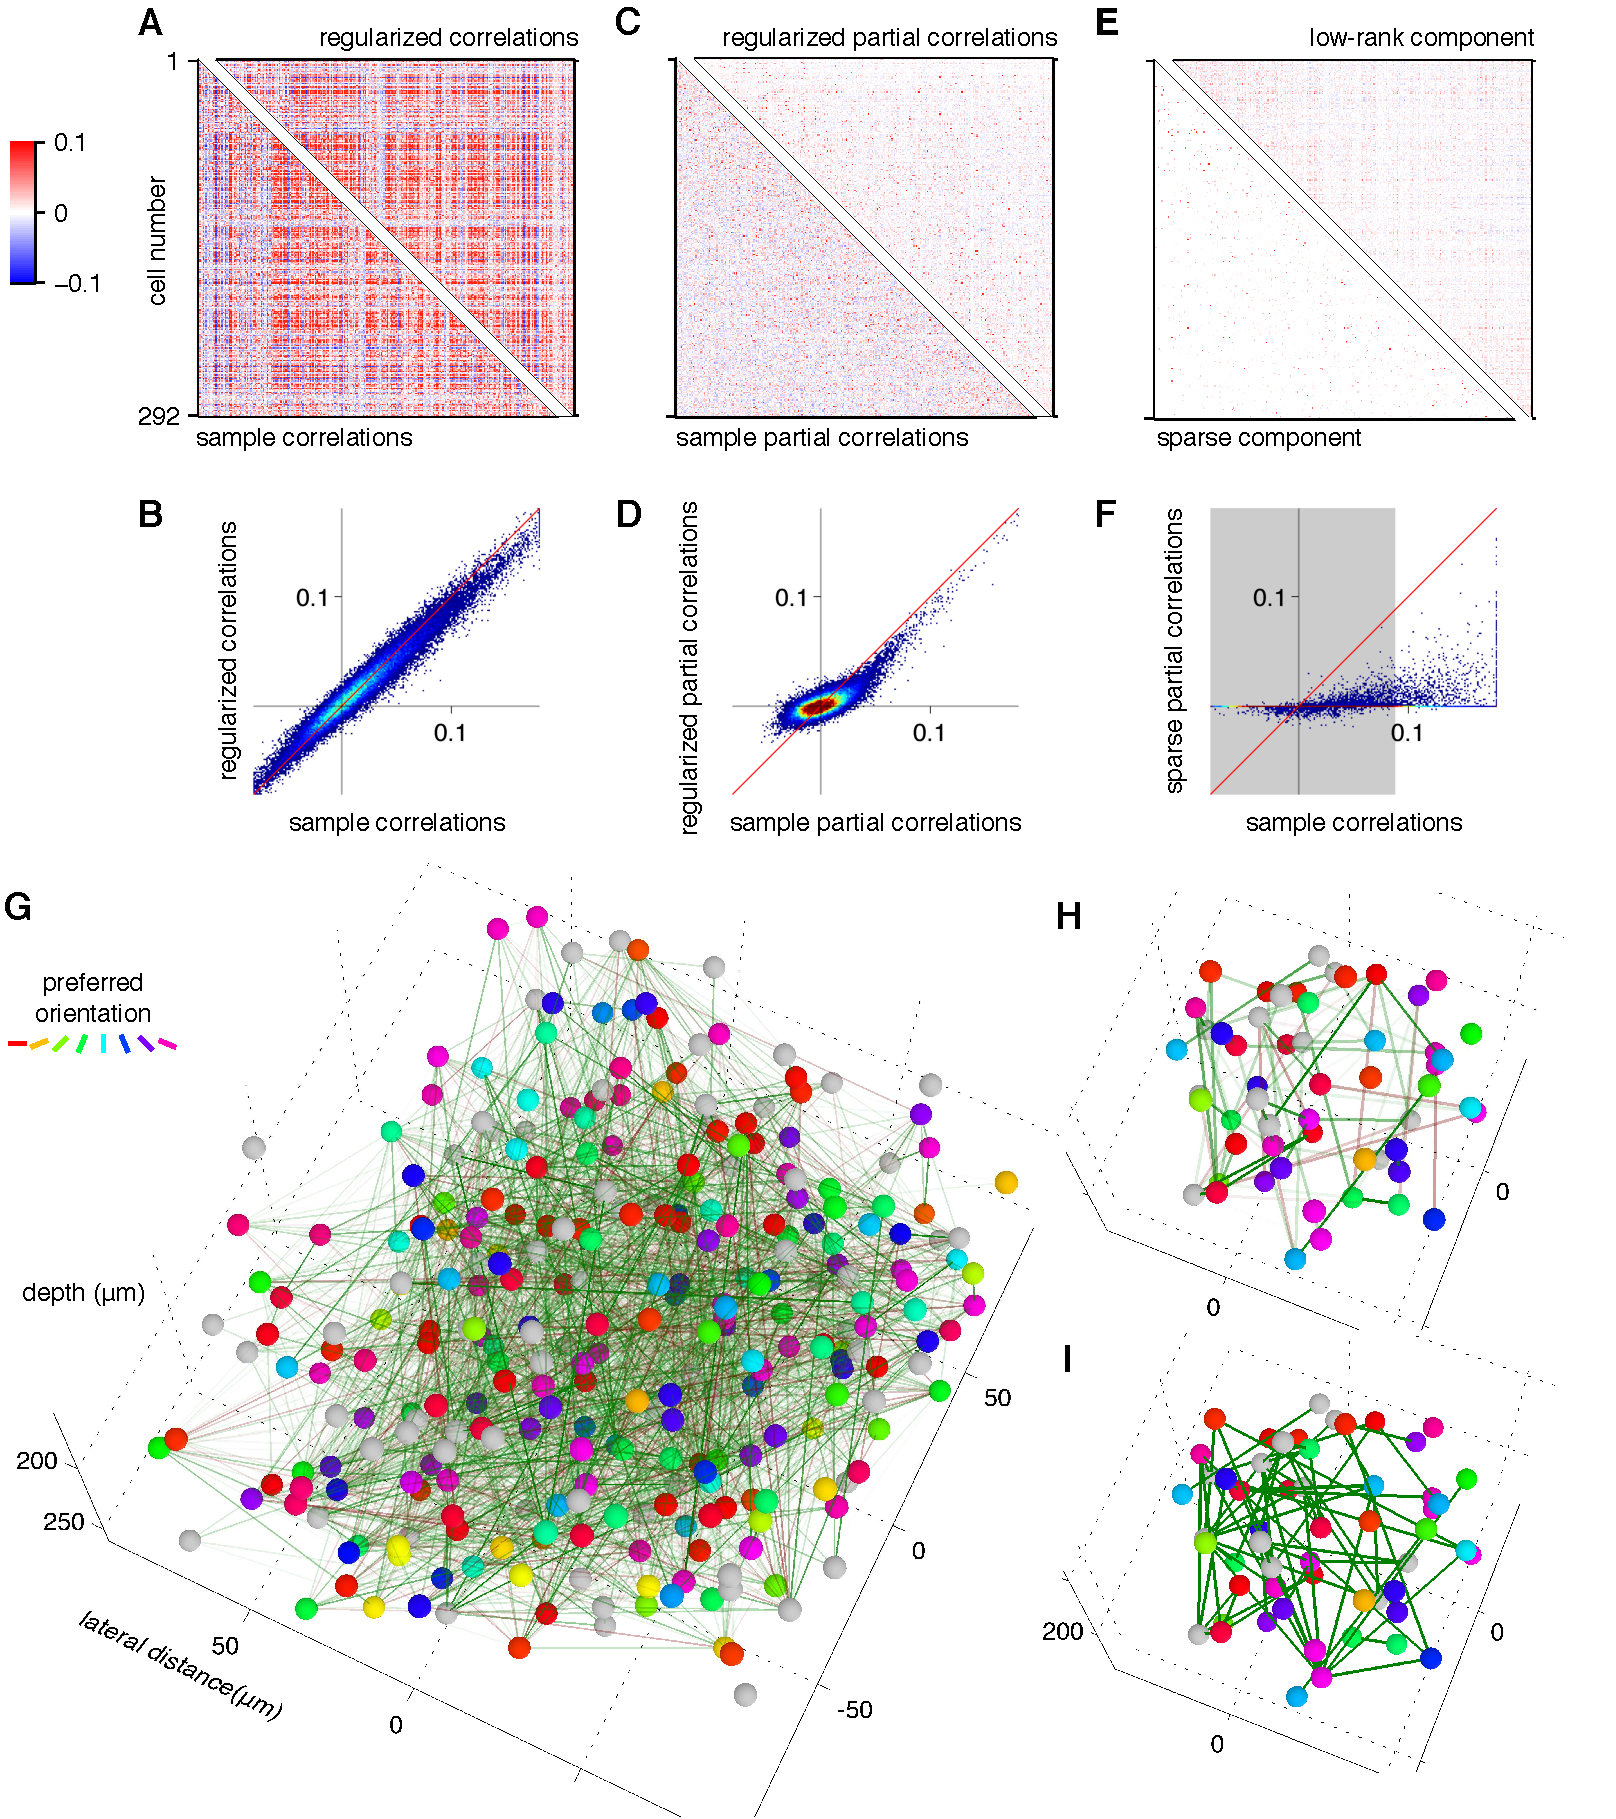
\includegraphics[height=\textwidth]{./figures/Reconstruction.pdf}
        \end{center}
\end{fullpage}
\end{figure}
   %%  Figure 4 from paper

\begin{figure}
\begin{fullpage}

\begin{center}
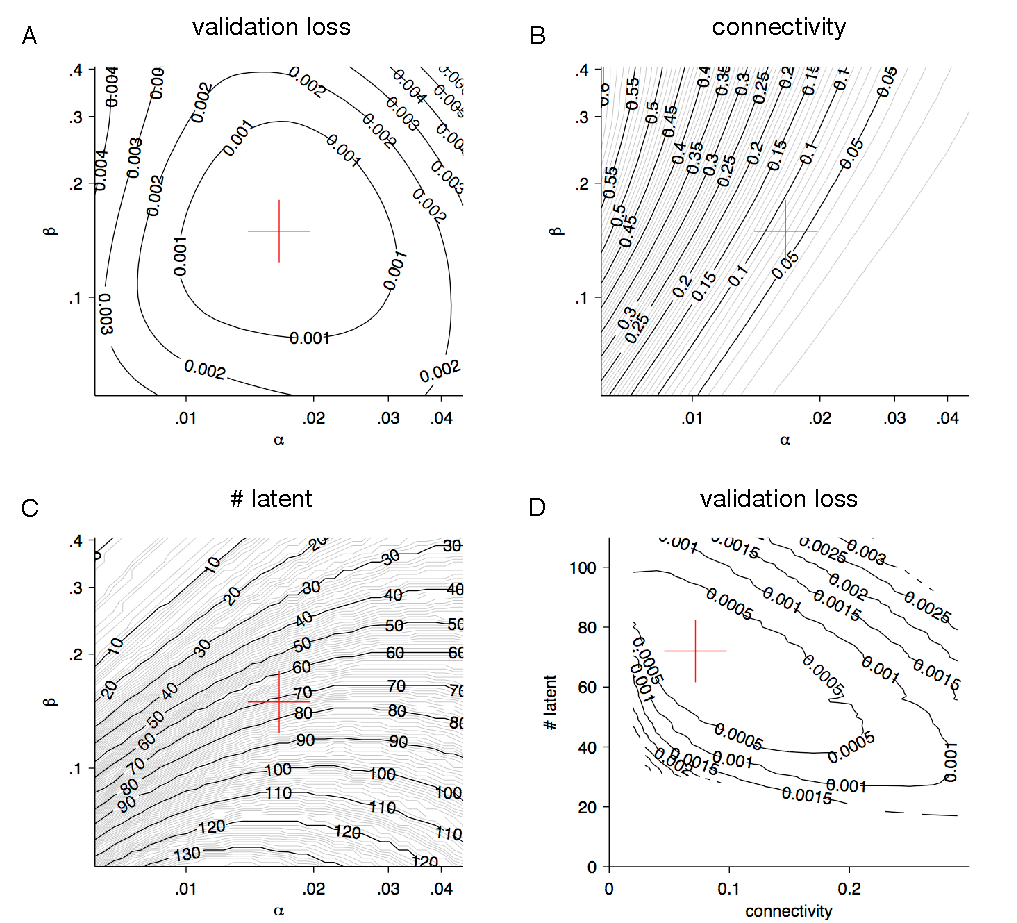
\includegraphics[width=\textwidth]{./figures/Supp1.pdf}
\end{center}

\caption[Optimization of regularization parameters]{
{\bf Optimization of regularization parameters of the $C_{\sf sparse+latent}$ estimator.} {\bf A.} Validation loss (Eq.~\ref{eq:full-loss}) for the example site in Fig.~\ref{fig:2} and \ref{fig:4} as a function of the hyperparameters $\alpha$ and $\beta$ of the $C_{\sf sparse+latent}$ estimator (Eq.~\ref{eq:c-sl} and Eq.~\ref{eq:ma}). In all panels, the red cross marks the optimal value found by the pattern search algorithm described in Methods.
{\bf B.} The connectivity ($1-\mbox{sparsity}$) of the sparse component $S$ as a function of $\alpha$ and $\beta$ for the example site.
{\bf C.} The number of latent units, \emph{i.e.}~the rank of the low-rank component $L$, as a function of hyperparameters $\alpha$ and $\beta$.
{\bf D.} The loss function as a function of the connectivity and the number of latent units.
}\label{fig:S1}
\end{fullpage}
\end{figure}   %% Figure S1 from paper

To test this hypothesis, we computed the relative validation loss of estimators  $C_{\sf sample}$, $C_{\sf diag}$, $C_{\sf factor}$, and $C_{\sf sparse}$ with respect to $C_{\sf sparse+latent}$ in $n=27$ imaged sites in 14 mice.  The hyperparameters of each estimator were optimized by nested cross-validation (See Fig.~\ref{fig:S1} and  Methods). Indeed, the sparse+latent estimator outperformed the other estimators (Fig.~\ref{fig:4}). The respective median differences of the validation loss were 0.039, 0.0016, 0.0029, and 0.0059 nats/cell/bin, significantly greater than zero ($p<0.01$ in each comparison, $n=27$ sites in 14 mice, Wilcoxon signed rank test).

\subsection*{Structure of $C_{\sf sparse+latent}$ estimates}

\begin{figure}
\begin{fullpage}
    \begin{center}
        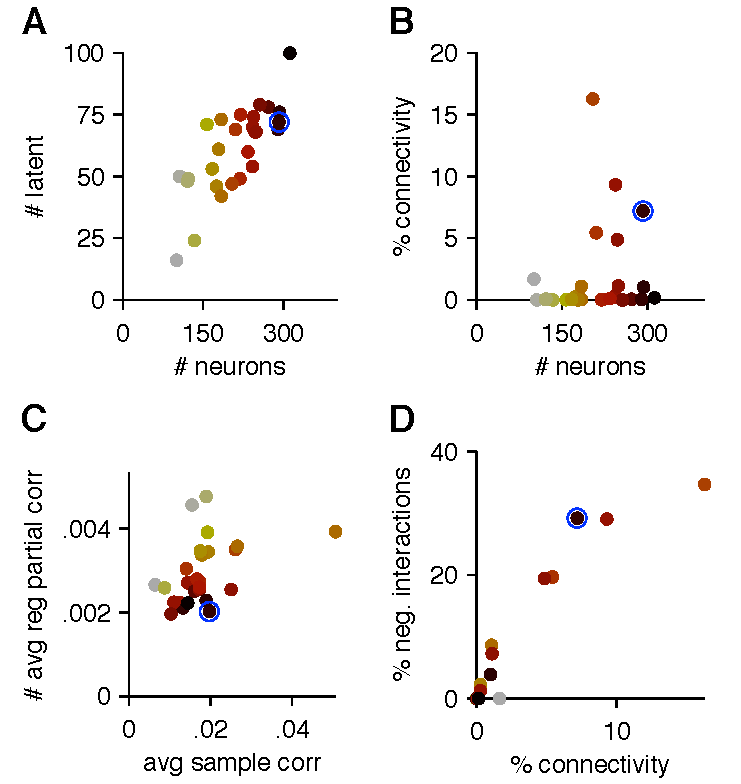
\includegraphics{./figures/Stats.pdf}
    \end{center}

\begin{caption}[Properties of functional connectivity across datasets]
{\bf Properties of functional connectivity across datasets.}
Each point represents an imaged site with its color indicating the population size as shown in panels A and B. The example site from Figures \ref{fig:2} and \ref{fig:4} is circled in blue.
\\
{\bf A.} The number of inferred latent units \emph{vs.}~population size.
{\bf B.} The connectivity of the sparse component of partial correlations as a function of population size.
{\bf C.} The average sample correlations \emph{vs.}~the average partial correlations (Eq.~\ref{eq:partial}) of the $C_{\sf sparse+latent}$ estimate.
{\bf D.} The percentage of negative interactions vs.~connectivity in the $C_{\sf sparse+latent}$ estimates.

\end{caption} \label{fig:5}

\end{fullpage}
\end{figure}
   %%  Figure 5 from paper

\begin{figure}
\begin{fullpage}
    \begin{center}
        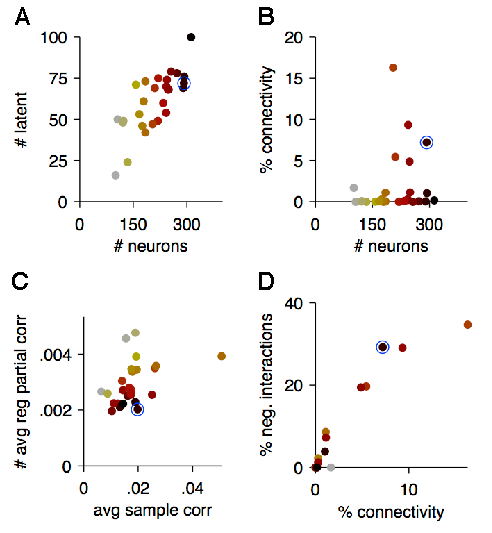
\includegraphics{./figures/Figure6.pdf}
    \end{center}

\caption[Properties of $C_{\sf sparse+latent}$ estimates]
{
{\bf Properties of $C_{\sf sparse+latent}$ estimates from all imaged sites.}
Each point represents an imaged site with its color indicating the population size as shown in panels A and B. The example site from Figures \ref{fig:3} and \ref{fig:5} is circled in blue.
\\
{\bf A.} The number of inferred latent units \emph{vs.}~population size.
{\bf B.} The connectivity of the sparse component of partial correlations as a function of population size.
{\bf C.} The average sample correlations \emph{vs.}~the average partial correlations (Eq.~\ref{eq:partial}) of the $C_{\sf sparse+latent}$ estimate.
{\bf D.} The percentage of negative interactions vs.~connectivity in the $C_{\sf sparse+latent}$ estimates.
}\label{fig:6}

\end{fullpage}
\end{figure}   %%  Figure 6 from paper


We examined the composition of the $C_{\sf sparse+latent}$ estimates at each imaged site (Fig.~\ref{fig:5} and Fig.~\ref{fig:6}). Although the regularized estimates were similar to the sample correlation matrix (Fig.~\ref{fig:5} A and B), the corresponding partial correlation matrices differed substantially (Fig.~\ref{fig:5} C and D). The estimates separated two sources of correlations: a network of linear interactions expressed by the sparse component of the inverse and latent units expressed by the low-rank components of the inverse (Fig.~\ref{fig:5} E). The sparse partial correlations revealed a network that differed substantially from the network composed of the greatest coefficients in the sample correlation matrix (Fig.~\ref{fig:5} F, G, H, and I).

In the example site (Fig.~\ref{fig:5}), the sparse component had 92.8\% sparsity (or conversely, 7.2\% connectivity: $\mbox{connectivity}=1-\mbox{sparsity}$) with average node degree of 20.9 (Fig.~\ref{fig:5} G). The average node degree, \emph{i.e.}\;the average number of interactions linking each neuron, is related to connectivity as $\mbox{degree} = \mbox{connectivity}\cdot(p-1)$, where $p$ is the number of neurons. The low-rank component had rank 72, denoting 72 inferred latent units. The number of latent units increased with population size (Fig.~\ref{fig:6} A) but the connectivity was highly variable (Fig.~\ref{fig:6} B): Several sites, despite their large population sizes, were driven by latent units and had few pairwise interactions. This variability may be explained by differences in brain states and recording quality and warrants further investigation.

The average partial correlations calculated from these estimates according to Eq.~\ref{eq:partial} at all 27 sites were about 5 times lower than the average sample correlations (Fig.~\ref{fig:6} C). This suggests that correlations between neurons build up from multiple chains of smaller interactions. Furthermore, the average partial correlations were less variable: the coefficient of variation of the average sample correlations across sites was 0.45 whereas that of the average partial correlations was 0.29, with larger populations exhibiting greater uniformity of average partial correlations than the smaller populations ($p=0.002$ Brown-Forsythe test).

While the sample correlations were mostly positive, the sparse component of the partial correlations (`interactions') had a high fraction (28.7\% in the example site) of negative values (Fig.~\ref{fig:5} F). The fraction of negative interactions increased with the inferred connectivity (Fig.~\ref{fig:6} D), suggesting that negative interactions can be inferred only after a sufficient density of positive interactions has been uncovered.

Thresholded sample correlations have been used in several studies to infer pairwise interactions \citep{Golshani:2009, Feldt:2011, Malmersjo:2013, Sadovsky:2014}.  We therefore compared the interactions in the sparse component of $C_{\sf sparse+latent}$ to those obtained from the sample correlations thresholded to the same level of connectivity. The networks revealed by the two methods differed substantially. In the example site with 7.2\% connectivity in $C_{\sf sparse+latent}$, only 27.7\% of the connections coincided with the above-threshold sample correlations (Fig.~\ref{fig:5} F, H, and I). In particular, most of the inferred negative interactions corresponded to low sample correlations (Fig.~\ref{fig:5} F) where high correlations should be expected given the rest of the correlation matrix.

\subsection*{Relationship of $C_{\sf sparse+latent}$ to orientation tuning and physical distances}

\begin{figure}
\begin{fullpage}
        \begin{center}
        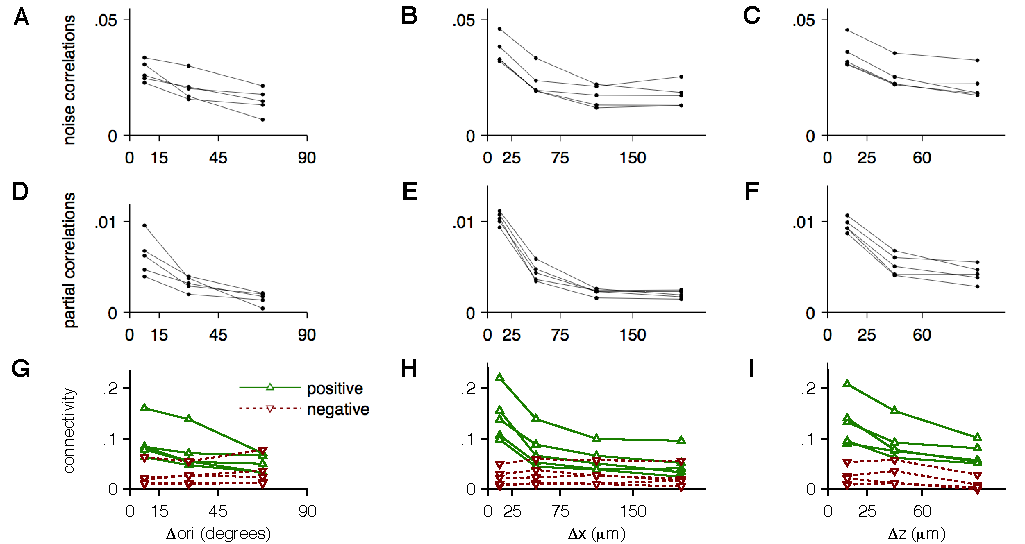
\includegraphics[width=\textwidth]{./figures/Figure7.pdf}
        \end{center}
        
\caption[Relationship between functional connectivity and circuit architecture]{
{\bf Relationship between functional connectivity and circuit architecture}
Dependence of sample correlations, regularized partial correlations, and connectivity inferred by $C_{\sf sparse+latent}$ on the differences in preferred orientations, $\Delta \mbox{ori}$, and physical distances: horizontal $\Delta x$ and depth $\Delta z$.
Five sites with highest connectivity (see Fig.~\ref{fig:6} B) were selected for this analysis.
\\
{\bf A--C.} Mean sample correlations in relation to $\Delta\mbox{ori}$,  $\Delta x$ and $\Delta z$, respectively. For $\Delta x$ averages, only horizontally aligned cell pairs with $\Delta z<30\,\mu m$ were considered. Similarly, for $\Delta z$ averages, only vertically aligned cell pairs with $\Delta x<30\,\mu m$ were considered.
\\
{\bf D--F.} Mean partial correlations regularized by the $C_{\sf sparse+latent}$ estimator binned the same way as the sample correlations above. The partial correlations exhibit stronger dependence on $\Delta\mbox{ori}$, $\Delta x$, and $\Delta z$ than sample correlations. 
\\
{\bf G--I.} Positive connectivity (green) and negative connectivity (red) inferred by the $C_{\sf sparse+latent}$ estimator. 
Positive and negative connectivities refer to the fractions of the positive and negative partial correlations computed from the sparse component $S$ of $C_{\sf sparse+latent}$.  
Positive connectivity decreases with $\Delta \mbox{ori}$, $\Delta x$, and $\Delta z$. 
Negative connectivity does not decrease with $\Delta \mbox{ori}$, $\Delta x$ within the examined range, and with $\Delta z$ for small values of $\Delta z<60\,\mu m$.
}\label{fig:7}

\end{fullpage}
\end{figure}
  %%  Figure 7 from paper

We examined how the structure of the $C_{\sf sparse+latent}$ estimates related to the differences in orientation preference and to the physical distances separating pairs of cells (Fig.\;\ref{fig:7}).  Five sites with highest pairwise connectivities were included in the analysis. Partial correlations were computed using Eq.~\ref{eq:partial} based on the regularized estimate, including both the sparse and the latent component. Connectivity was computed as the fraction of pairs of cells connected by non-zero elements (interactions) in the sparse component of the estimate, distinguishing between the positive and negative connectivities.

First, we analyzed how correlations and connectivity depended on the difference in preferred orientations ($\Delta \mbox{ori}$) of pairs of significantly ($\alpha=0.05$) tuned cells. The partial correlations decayed more rapidly with $\Delta\mbox{ori}$ than did sample correlations ($p<10^{-9}$ in each of the five sites, two-sample $t$-test of the difference of the linear regression coefficients). Positive connectivity decreased with $\Delta\mbox{ori}$ ($p<0.005$ in each of the five sites, $t$-test on the logistic regression coefficient) whereas negative connectivity did not decrease (Fig.~\ref{fig:7} D): The slope in the logistic model of connectivity with respect to $\Delta\mbox{ori}$ was significantly higher for positive than for negative interactions ($p<0.04$ in each of the five sites, two-sample $t$-test of the difference of the logistic regression coefficient).

Second, we compared how correlations and connectivity depended on the physical distance separating pairs of cells. We distinguished between lateral distance, $\Delta x$, in the plane parallel to the pia, and vertical distance, $\Delta z$, orthogonal to the pia.  When considering the dependence on $\Delta x$, the analysis was limited to cell pairs located at the same depth with $\Delta z < 30\,\mu\mbox{m}$; conversely, when considering the dependence on $\Delta z$, only vertically aligned cell pairs with $\Delta x < 30\,\mu\mbox{m}$ were included. Again, the partial correlations decayed more rapidly both laterally and vertically than sample correlations ($p<10^{-6}$ in each of the five sites, for both lateral and vertical distances, two-sample $t$-test of the difference of the linear regression coefficients).
Positive connectivity decayed with distance ($p<10^{-6}$ in each of the five sites for positive interactions and $p<0.05$ for negative interactions, $t$-test on the logistic regression coefficient) (Fig.~\ref{fig:7} E), so that cells separated laterally by less than 25 $\mu\mbox{m}$ were 3.2 times more likely to be connected than cells separated laterally by more than 150 $\mu\mbox{m}$. Although the positive connectivity appeared to decay faster with vertical than with lateral distance, the differences in slopes of the respective logistic regression models were not significant with available data. The negative connectivity decayed slower with distance (Fig.~\ref{fig:7} E and F): The slope in the respective logistic models with respect to the lateral distance was significantly higher for positive than for negative connectivities ($p<0.05$ in each of the five sites, two-sample $t$-test of the difference of the logistic regression coefficients).